\documentclass[./main.tex]{subfiles} 
\begin{document}

\subsection{A Real Time Spectrum Analyser Using Least Mean Square}

\subsubsection{DFT-CLMS}

The DFT-CLMS was implemented using the CLMS filter, and the data from the estimated AR coefficients passed on. Figure \ref{fig:4_3_c} shows the DFT-CLMS and esimated frequency output. It clearly does not appear quite like the spectrogram previously seen. Fundamentally, the DFT runs with a set of data each sample contributes in some fashion to each frequency bin. The CLMS algorithm runs in sequential order and thus is unable to explore each time sample to update each weight in the same fashion the DFT is.

\begin{figure}[h]
	\centering 
	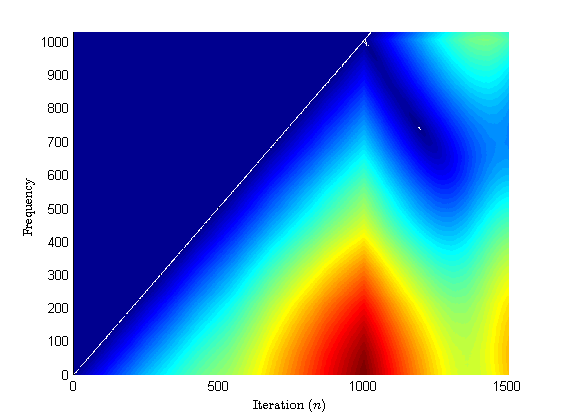
\includegraphics[scale=1]{fig/4/4_3_c.png}
	\caption{\textit{DFT-CLMS of spectrum from the AR estimator}}
	\label{fig:4_3_c}
\end{figure}

\end{document}

